\documentclass[11pt,a4paper,draft]{article}
\usepackage[utf8]{inputenc}
\usepackage[margin=1in]{geometry}
\usepackage{graphicx}
\setlength{\headheight}{14pt}
\addtolength{\topmargin}{-2pt}
\usepackage{amsmath}
\usepackage{amssymb}
\usepackage{hyperref}
\usepackage{booktabs}
\usepackage{caption}
\usepackage{subcaption}
\usepackage{float}
\usepackage{enumitem}
\usepackage{fancyhdr}
\usepackage{titlesec}
\usepackage{listings}
\usepackage{xcolor}
\usepackage{algorithm}
\usepackage{algpseudocode}

% Code listing style
\lstset{
    basicstyle=\ttfamily\small,
    keywordstyle=\color{blue},
    commentstyle=\color{green!60!black},
    stringstyle=\color{red},
    showstringspaces=false,
    breaklines=true,
    frame=single,
    numbers=left,
    numberstyle=\tiny\color{gray}
}

% Header and Footer Setup
\pagestyle{fancy}
\fancyhf{}
\rhead{Group 3 -- Final Report}
\lhead{Beko Europe Project}
\rfoot{Page \thepage}

\begin{document}

% =============================================================================
% TITLE PAGE
% =============================================================================
\begin{titlepage}
    \centering
    \thispagestyle{empty}

    \vspace*{1cm}
    
    
\includegraphics[width=0.35\textwidth]{polimi_logo.png} 
    
    \vspace{1.0cm}
    
    {\Large \textsc{Politecnico di Milano}\\ 
    Department of Electronics, Information and Bioengineering (DEIB)\par}
    
    \vspace{3cm}
    
    {\Huge \textbf{Automated Visual Inspection System for PCB Connectors}\par}
    \vspace{0.5cm}
    {\Large \textbf{Project Work Report -- Beko Europe}\par}
    \vspace{0.5cm}
    {\large Academic Year 2025--2026\par}
    
    \vspace{3cm}
    
    {\large \textbf{Authors:}\par}
    \vspace{0.2cm}
    {\large
    Giovanni Passuello\\
    Karim Negm\\
    Feruzakhon Sulaymonova\\
    Tingyu Chen\par}
    
    \vspace{1.5cm}
    
    {\large \textbf{Supervisor:} Prof. Fredy Ruiz\par}
    \vspace{0.1cm}
    {\large \textbf{Co-advisors:} Marco Cederle, Davide Cazzaniga\par}
    
    \vfill
    
    {\large February 2026\par}
    
\end{titlepage}

\newpage

% =============================================================================
% TABLE OF CONTENTS
% =============================================================================
\tableofcontents
\newpage

% =============================================================================
% REPORT BODY
% =============================================================================

\section{Executive Summary}

This report presents the development of an automated visual inspection system for PCB connector assemblies at Beko Europe. The final deliverable is a deployable software pipeline capable of detecting missing cable connections with \textbf{95.13\% overall accuracy} across nine connector types and 2{,}853 images.

The core technical challenge is extreme class imbalance: genuine defects (KO) constitute less than 1\% of the dataset, making standard supervised classification impractical. Our solution reframes the problem as binary presence detection using \textbf{synthetic negative generation via inpainting}. For each connector, a polygon mask defines the expected cable region; OpenCV inpainting removes the cable content from real OK images to produce realistic synthetic KO samples on the fly. 

We train a per-connector ResNet18 classifier on these real/synthetic pairs. The model outputs a continuous $P_{\mathrm{KO}}$ score, calibrated using a percentile-based threshold on real OK validation data. This score supports both binary decisions and operator-facing confidence displays.

This architecture supersedes earlier exploration of PatchCore (memory-intensive, slow inference) and EfficientAD (inconsistent recall across connectors), both of which struggled with the three-class OK/KO/OCCLUSION problem. The final pipeline is lightweight, reproducible and maintainable for long-term factory deployment.

\section{Introduction and Problem Statement}

\subsection{Industrial Context}

For Beko Europe, ensuring secure PCB connections is a critical safety and reliability imperative. A missing connector detected at final electrical testing requires \textbf{full appliance reassembly}, creating significant production bottlenecks. Internal analysis indicates these failures occur predominantly in the \textbf{upper panel assembly}, making this area the focus of automated monitoring.

Traditional human inspection faces inherent limitations: operator fatigue over long shifts, high line speed allowing only brief inspection windows and visual obstructions from overlapping cables. The objective is to deploy an automated system as a consistent, complementary quality assurance layer that mitigates human error.

\subsection{Technical Challenges}

The task presents several non-trivial challenges from a machine learning perspective.

\textbf{Extreme class imbalance.} The dataset contains 2{,}853 connector images from 317 boards. Among these, only 25 are genuine KO cases (0.9\%), while 485 (17\%) are non-defective occlusions and 2{,}343 (82.1\%) are OK. A classifier trained naively on this distribution would simply predict OK for everything, achieving $>$99\% accuracy while missing all defects.

\textbf{Visual ambiguity from occlusions.} Cables from other connections frequently pass in front of connectors, partially or fully blocking the view. These occlusions are visually similar to missing cables yet are not defects. A naive anomaly detector flags both KO and OCCLUSION as anomalous, producing unacceptably high false positive rates.

\textbf{Illumination and perspective variability.} Small variations in board positioning, ambient lighting throughout the day and camera vibrations introduce variability that a robust system must handle gracefully. Morning-to-afternoon intensity variation was measured at 1.73 grayscale units before normalization.

\textbf{Limited training data.} With approximately 300 images per connector type and fewer than 5 true defects per connector, extended production line monitoring for data collection has practical and economic limitations.

\subsection{Project Objectives}

The primary objective is to reliably detect the presence or absence of cable connections under real industrial conditions. We emphasize minimizing false negatives, since undetected defects represent higher operational risk than triggering additional human inspection. The system must be deployable on standard industrial PCs without GPU infrastructure and scalable to different connector types without complete redesign.

The project scope intentionally excludes partial insertion detection. According to Beko engineers, connectors are mechanically designed to either accept cables correctly or reject them entirely; rare intermediate cases are handled by downstream electrical testing.


\section{System Design and Hardware}

\subsection{Camera Configuration}

Our initial approach considered stereo vision to provide depth information distinguishing cables passing in front of connectors from those actually inserted.

\begin{figure}[H]
    \centering
    \begin{subfigure}{0.48\textwidth}
        \includegraphics[width=\textwidth]{figures/stereo_setup_diagram.png}
        \caption{Stereo camera configuration}
    \end{subfigure}
    \hfill
    \begin{subfigure}{0.48\textwidth}
        \includegraphics[width=\textwidth]{figures/stereo_depth_map.png}
        \caption{Computed depth map}
    \end{subfigure}
    \caption{Stereo vision proof-of-concept}
    \label{fig:stereo_poc}
\end{figure}

A proof-of-concept demonstrated that depth maps could be computed effectively. However, consultation with Beko engineers revealed that stereo's advantages did not justify its mechanical complexity and calibration requirements, given that partial insertion detection was not required.

The final setup uses two fixed cameras with manual settings (ISO, exposure, white balance):

\begin{figure}[H]
    \centering
    \begin{subfigure}{0.48\textwidth}
        \includegraphics[width=\textwidth]{figures/camera_config_top.png}
        \caption{Top view (10\textdegree\ tilt)}
    \end{subfigure}
    \hfill
    \begin{subfigure}{0.48\textwidth}
        \includegraphics[width=\textwidth]{figures/camera_config_lateral.png}
        \caption{Rear camera (25--35\textdegree\ azimuth)}
    \end{subfigure}
    \caption{Final optimized camera placement}
    \label{fig:camera_final}
\end{figure}

\textbf{Top Camera:} Positioned vertically with 10\textdegree\ forward tilt to reduce reflections, clear the raised front panel (8--10\,cm height difference) and provide slight depth perspective for cable routing assessment.

\textbf{Rear Camera:} Horizontal mounting with 25--35\textdegree\ azimuthal rotation, critical for observing rear panel connectors that would be invisible from perpendicular angles.

Both cameras use fixed manual settings ensuring temporal consistency.

\subsection{Preprocessing Pipeline}

Raw images undergo a three-stage preprocessing pipeline before model input.

\textbf{Alignment.} Feature-based homography estimation using ORB features (4{,}000 keypoints, Hamming distance matching with RANSAC outlier rejection). If feature matching yields fewer than 15 correspondences, the system falls back to Enhanced Correlation Coefficient (ECC) optimization for dense alignment. This ensures connectors appear at consistent pixel locations across all images.

\begin{figure}[H]
    \centering
    \begin{subfigure}{0.48\textwidth}
        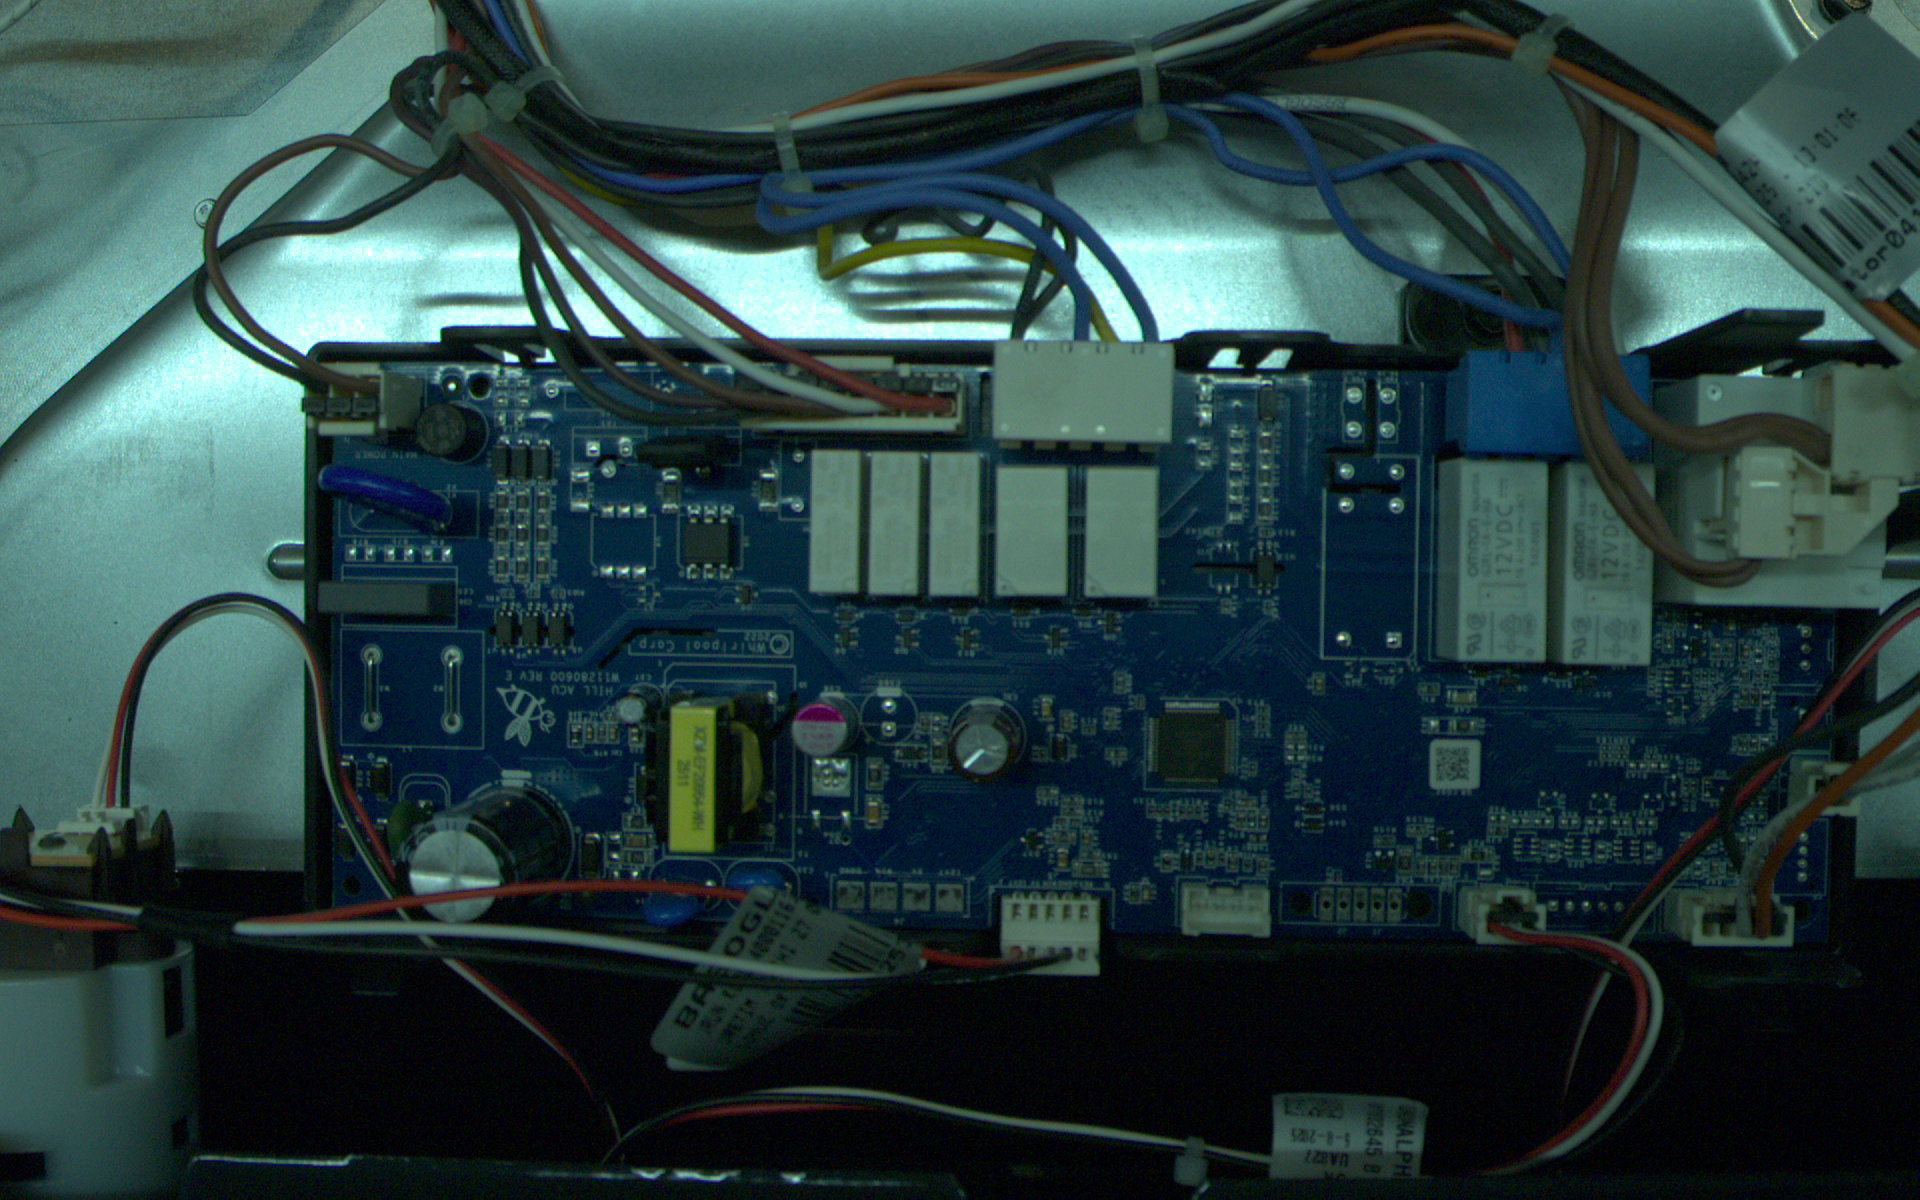
\includegraphics[width=\textwidth]{figures/raw_image_1.png}
        \caption{Before: varying positions}
    \end{subfigure}
    \hfill
    \begin{subfigure}{0.48\textwidth}
        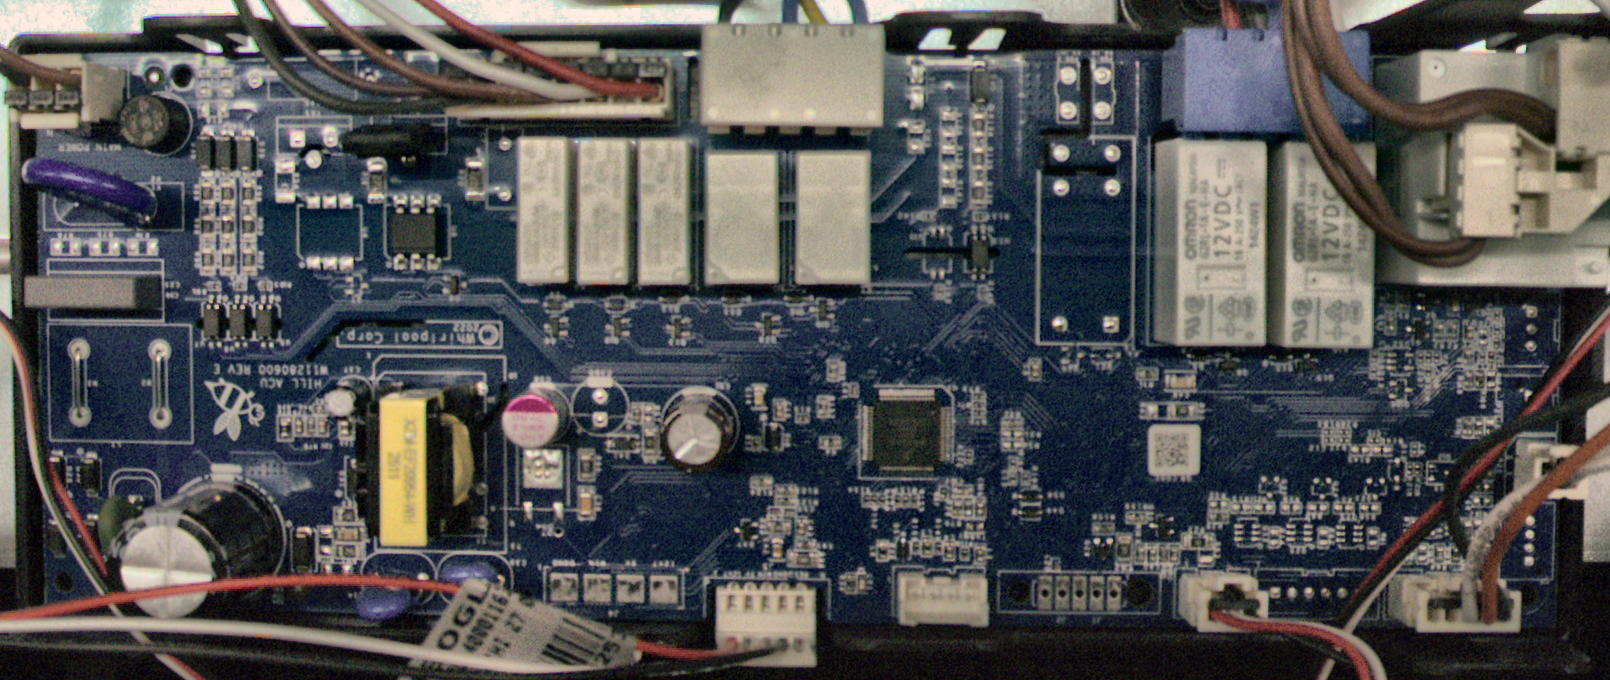
\includegraphics[width=\textwidth]{figures/aligned_image_1.png}
        \caption{After: consistent alignment}
    \end{subfigure}
    \caption{Image alignment preprocessing}
    \label{fig:alignment}
\end{figure}

\textbf{Illumination normalization.} To handle lighting variations throughout the day, we apply a two-stage approach. First, CLAHE (Contrast Limited Adaptive Histogram Equalization) enhances local contrast in the LAB color space. Second, gray-world white balance corrects color casts. This reduced morning-to-afternoon intensity variation by 68\%, from 1.73 to 0.54 grayscale units.

\textbf{Connector extraction.} Nine connector ROIs are defined using relative coordinates stored in \texttt{roi\_config.json}, enabling resolution independence. Each crop undergoes local CLAHE enhancement and is stored as a grayscale image for model input.

\begin{figure}[H]
    \centering
    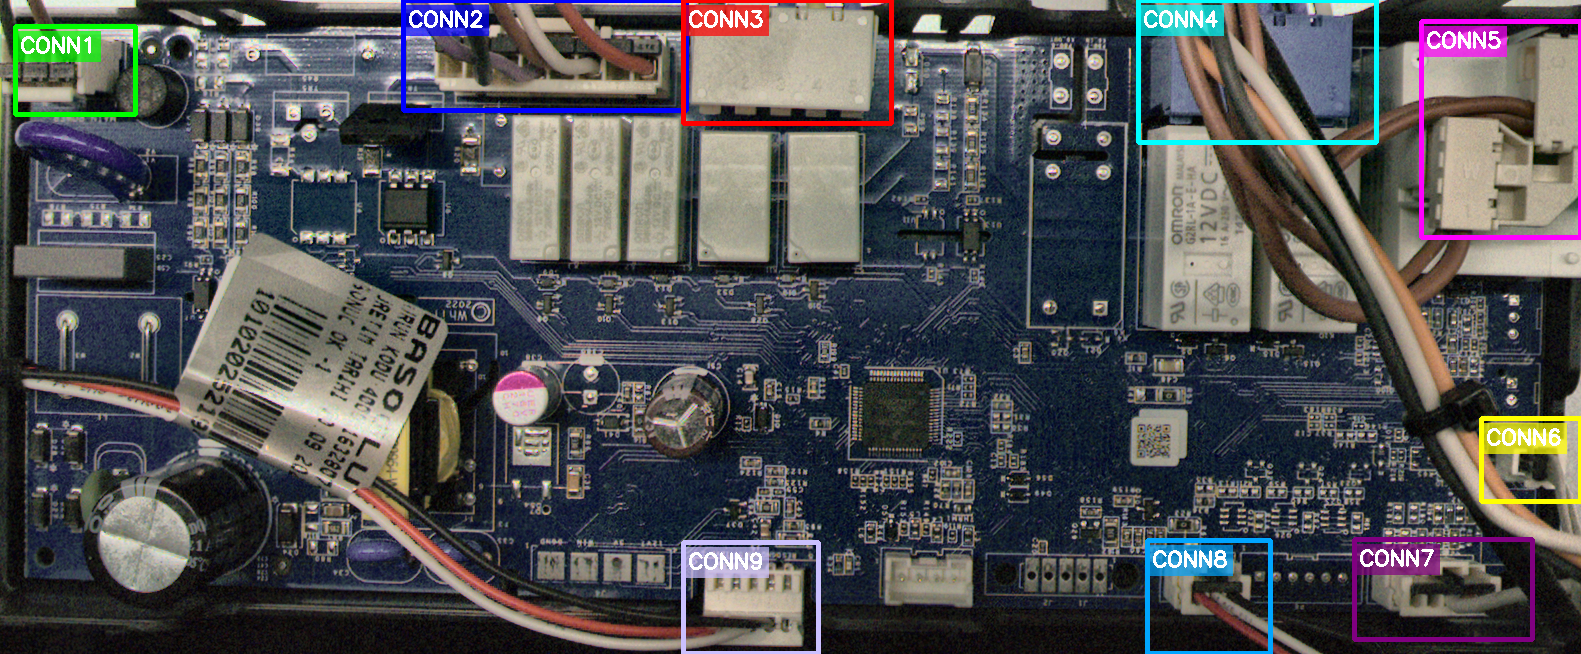
\includegraphics[width=0.9\textwidth]{figures/roi_visualization.png}
    \caption{Nine connector regions (CONN1--CONN9) extracted for analysis}
    \label{fig:rois}
\end{figure}



% CHAPTER 4 -- THE FINAL SOLUTION (MOVED UP FOR EMPHASIS)
% =============================================================================
\section{Solution: Synthetic Negative Detection}

This section describes the final training and inference pipeline implemented in \texttt{pcl\_presence\_training.ipynb}. The key insight is to convert the rare-defect problem into a standard supervised learning task by generating realistic synthetic negatives through inpainting within connector-specific masks.

\subsection{Problem Reframing and Rationale}

For each connector crop, the decision is reduced to a binary presence check: is the PCL (cable) present or absent in the expected region? This framing matches the actual manufacturing requirement. Beko engineers confirmed that the failure mode of interest is missing connections, not partial seating depth. 

The advantage of this formulation is fundamental: instead of requiring a collection of rare real KO samples (of which we have fewer than 5 per connector), we generate unlimited synthetic KO examples by programmatically removing the cable from real OK images. The classifier learns the visual signature of ``cable present'' versus ``cable absent'' using matched pairs derived from the same source image. This avoids mismatches between training and real data that would arise from using generic augmentation.

\subsection{Mask-Driven Synthetic KO Generation}

Each connector has a dedicated polygon mask stored in \texttt{mask\_config.json} that delineates the expected PCL region. Masks are defined using relative coordinates (invariant to image resolution) and converted to binary arrays matching the crop dimensions. The synthetic KO generation procedure operates as follows.

Given a real OK crop $\mathbf{x}_{\mathrm{OK}} \in \mathbb{R}^{H \times W}$ and binary mask $\mathbf{M} \in \{0, 1\}^{H \times W}$:

\begin{enumerate}[nosep]
    \item \textbf{Mask dilation.} The mask is dilated by $d$ pixels (default $d=3$) using a $(2d+1) \times (2d+1)$ square kernel to ensure full PCL coverage at boundaries:
    \begin{equation}
        \mathbf{M}_d = \mathbf{M} \oplus \mathbf{K}_d
    \end{equation}
    where $\oplus$ denotes morphological dilation.
    
    \item \textbf{Inpainting.} The masked region is reconstructed using OpenCV's Telea inpainting~\cite{telea2004inpainting} (or Navier-Stokes variant), which propagates surrounding texture into the masked area:
    \begin{equation}
        \mathbf{x}_{\mathrm{inp}} = \mathrm{Inpaint}(\mathbf{x}_{\mathrm{OK}},\; \mathbf{M}_d,\; r)
    \end{equation}
    where $r$ is the inpainting radius (default $r=3$).
    
    \item \textbf{Boundary blending.} A Gaussian-blurred alpha mask ($\sigma=5$, kernel $15 \times 15$) provides smooth transitions at mask boundaries:
    \begin{equation}
        \mathbf{x}_{\mathrm{KO}} = \alpha \cdot \mathbf{x}_{\mathrm{inp}} + (1 - \alpha) \cdot \mathbf{x}_{\mathrm{OK}}, \quad \alpha = G_\sigma(\mathbf{M}_d)
    \end{equation}
\end{enumerate}

To improve diversity across training epochs, key parameters are randomized at each sample generation: the inpainting radius is scaled by a factor drawn from $\mathcal{U}(0.8, 1.2)$, the dilation width is perturbed by $\{-1, 0, +1\}$ pixels and the inpainting method alternates between Telea (80\% probability) and Navier-Stokes (20\% probability).

\subsection{Dataset Construction and Augmentation}

The training dataset is constructed exclusively from real OK images. For each image file, the \texttt{PCLPresenceDataset} returns two samples: the original crop labelled OK ($y=0$) and a synthetic inpainted version labelled KO ($y=1$). This produces a perfectly balanced binary dataset without requiring any real KO annotations.

Light augmentations are applied to both classes during training to improve robustness to production variability: brightness jitter ($\times \mathcal{U}(0.9, 1.1)$), contrast jitter ($\times \mathcal{U}(0.9, 1.1)$), additive Gaussian noise ($\sigma=5$) and occasional Gaussian blur ($p=0.1$, kernel $3 \times 3$, $\sigma=0.5$). These transforms are applied after synthetic KO generation to ensure both classes experience identical augmentation distributions.

The dataset is split 90/10 into training and validation sets using a fixed random seed for reproducibility. The training dataloader uses shuffled sampling with batch size 32.

\subsection{Model Architecture}

The classifier is a ResNet18~\cite{he2016resnet} backbone pretrained on ImageNet, adapted for single-channel grayscale input:

\begin{itemize}[nosep]
    \item \textbf{Input:} $128 \times 128 \times 1$ grayscale crop, normalized to $[0, 1]$.
    \item \textbf{Modified first layer:} \texttt{Conv2d(1, 64, 7$\times$7, stride=2, padding=3)} replaces the original 3-channel input convolution.
    \item \textbf{Output head:} The final fully connected layer is replaced by \texttt{Linear(512, 1)}, producing a single logit.
\end{itemize}

The KO probability is computed via the sigmoid function:
\begin{equation}
    P_{\mathrm{KO}} = \sigma\bigl(f_\theta(\mathbf{x})\bigr) = \frac{1}{1 + \exp\bigl(-f_\theta(\mathbf{x})\bigr)}
\end{equation}
where $f_\theta(\mathbf{x})$ is the network logit output. The total parameter count is approximately 11.2M, all of which are trainable (no frozen layers). Per-connector specialization is essential because connector geometry, background texture and cable appearance differ significantly across the nine ROIs.

\subsection{Training Protocol}

Independent models are trained for each connector type using the following protocol:

\begin{itemize}[nosep]
    \item \textbf{Loss:} \texttt{BCEWithLogitsLoss} (numerically stable binary cross-entropy applied to raw logits).
    \item \textbf{Optimizer:} Adam with learning rate $10^{-4}$.
    \item \textbf{Epochs:} 15 maximum, with early stopping (patience = 5 epochs on validation loss).
    \item \textbf{Batch size:} 32.
    \item \textbf{Monitoring:} Validation AUC-ROC is computed at each epoch using \texttt{sklearn.metrics.roc\_auc\_score}.
\end{itemize}

At each epoch, the dataset's \texttt{set\_epoch()} method updates the random seed for synthetic KO generation, ensuring that the inpainting parameters vary across epochs and the model does not overfit to a single set of synthetic artefacts.

\subsection{Threshold Calibration}

A central design element is conservative threshold calibration using only real OK validation images. After training, inference is run on the validation OK set and the $P_{\mathrm{KO}}$ values are collected. The decision threshold $\tau$ is set as a high percentile of this distribution:
\begin{equation}
    \tau = \mathrm{Percentile}_{p}\bigl(\{P_{\mathrm{KO}}^{(i)}\}_{i \in \mathcal{V}_{\mathrm{OK}}}\bigr), \quad p = 99.5
\end{equation}

This guarantees that approximately 0.5\% of real OK validation samples exceed $\tau$, directly controlling the expected false positive rate under the validation distribution. The threshold is connector-specific: connectors with higher visual variability naturally yield higher $\tau$ values.

This calibration provides an operational control knob: increasing $p$ reduces false positives at the cost of reduced sensitivity; decreasing $p$ improves sensitivity at the cost of more false alarms. Crucially, adjusting $\tau$ does not require retraining.

\subsection{Inference Workflow}

At inference time, the per-connector decision follows a simple three-step routine:

\begin{enumerate}[nosep]
    \item Extract the connector crop from the aligned PCB image.
    \item Compute $P_{\mathrm{KO}} = \sigma(f_\theta(\mathbf{x}))$ using the corresponding per-connector model.
    \item Compare to the calibrated threshold:
\end{enumerate}
\begin{equation}
    \hat{y} =
    \begin{cases}
    \mathrm{KO} & \text{if } P_{\mathrm{KO}} \geq \tau \\
    \mathrm{OK} & \text{otherwise}
    \end{cases}
\end{equation}

The continuous $P_{\mathrm{KO}}$ value is displayed to operators alongside the binary decision, enabling manual review of borderline cases. For each connector, the pipeline saves trained weights (\texttt{model.pt}), the calibrated threshold with estimated FPR (\texttt{threshold.json}) and a training configuration summary (\texttt{training\_config.json}).

\subsection{Design Rationale and Key Decisions}

Several design choices distinguish this approach from standard supervised classification:

\textbf{Why inpainting over other augmentations?} Traditional data augmentation (rotation, scaling, color jitter) cannot synthesize the visual signature of a missing cable. Inpainting explicitly removes the cable region while preserving the surrounding connector geometry and background texture, creating realistic negative samples that match the true defect distribution.

\textbf{Why per-connector models?} Connector geometry, cable routing, background clutter and lighting conditions vary significantly across the nine ROIs. A shared global model would be dominated by easy cases (e.g.\ conn8 with high contrast) and fail on hard cases (e.g.\ conn6 with small PCL region). Per-connector specialization allows each model to learn the specific visual features relevant to its ROI.

\textbf{Why 99.5th percentile threshold?} The percentile-based calibration directly controls the expected false positive rate. Setting $p=99.5$ ensures that approximately 0.5\% of OK validation samples are flagged as KO, balancing sensitivity (minimizing missed defects) against specificity (minimizing false alarms). This threshold can be adjusted post-training without retraining, enabling operational tuning by plant engineers.

\textbf{Why grayscale input?} Preliminary experiments showed that cable presence is primarily a structural feature (edges, shadows, cavity depth) rather than a color feature. Grayscale input reduces model complexity (1 channel vs.\ 3), accelerates training and inference, and improves robustness to illumination color shifts (e.g.\ morning vs.\ afternoon lighting).




% =============================================================================
% CHAPTER 5 -- RESULTS (MOVED UP AFTER SOLUTION)
% =============================================================================
\section{Results and Performance Analysis}

\subsection{Overall Performance}

The final pipeline was evaluated on all 2{,}853 connector crops extracted from 317 aligned PCB images. For each connector, the corresponding per-connector model and calibrated threshold were applied.

\begin{table}[H]
\centering
\begin{tabular}{lcc}
\toprule
Metric & Value & Notes \\
\midrule
Total images & 2{,}853 & 9 connectors $\times$ 317 boards \\
Correct predictions & 2{,}714 & Across all labels \\
Overall accuracy & 95.13\% & Production-oriented calibration \\
\bottomrule
\end{tabular}
\caption{Overall system performance.}
\label{tab:overall}
\end{table}

\subsection{Per-Connector Breakdown}

Performance varies across connectors, reflecting differences in geometry, background complexity and occlusion frequency.

\begin{table}[H]
\centering
\small
\begin{tabular}{lccl}
\toprule
Connector & Accuracy & Correct/Total & Notes \\
\midrule
conn1 & 97.16\% & 308/317 & Stable background, strong mask quality \\
conn2 & 98.11\% & 311/317 & Clear PCL region, consistent lighting \\
conn3 & 100.00\% & 317/317 & Highest separability in probability space \\
conn4 & 94.01\% & 298/317 & Visual variability near mask boundary \\
conn5 & 96.85\% & 307/317 & Good separation with occasional ambiguity \\
conn6 & 88.01\% & 279/317 & Most challenging: subtle appearance changes \\
conn7 & 89.59\% & 284/317 & Sensitive to partial obstruction, reflections \\
conn8 & 98.11\% & 311/317 & Highly repeatable geometry and texture \\
conn9 & 94.32\% & 299/317 & Moderate difficulty with background clutter \\
\bottomrule
\end{tabular}
\caption{Per-connector performance of the presence detector pipeline.}
\label{tab:per_connector}
\end{table}

Connectors 3, 2 and 8 achieve near-perfect accuracy ($\geq$98\%), benefiting from stable geometry, minimal occlusion exposure and clear visual contrast between cable-present and cable-absent states. Connectors 6 and 7 represent the most challenging cases (88--90\% accuracy), where the PCL region is small relative to background clutter, reflections affect the masked region and illumination gradients reduce the visual signal that distinguishes OK from KO.

\subsection{Probability-Based Diagnostics}

Because the model outputs a continuous $P_{\mathrm{KO}}$ value, we can analyse separation quality beyond binary accuracy. For each connector, histograms of $P_{\mathrm{KO}}$ for OK and KO samples are plotted with the calibrated threshold $\tau$ overlaid. Clean separation (no histogram overlap) indicates high confidence. Overlap indicates borderline cases that would benefit from: (1) refined masks, (2) improved camera stability, or (3) expanded training data.

The Grad-CAM~\cite{selvaraju2017gradcam} saliency maps computed on ResNet18's \texttt{layer4} confirm that the model attends to the mask-defined PCL region for both OK and KO predictions. This validates that the model focuses on actual cable features rather than spurious patterns.

\subsection{Error Analysis}

The dominant failure modes are consistent with the pipeline design.

\textbf{False KO predictions} arise primarily from illumination gradients and specular reflections affecting the masked region, causing the inpainted region to appear visually similar to the actual connector state. This accounts for the majority of errors on connectors 6, 7 and 9.

\textbf{Missed KO predictions} occur when the PCL region is barely distinguishable even for human inspectors, typically due to near-background-colour cables or partial visibility of the connector.

\textbf{Mask imprecision} contributes to errors when the true cable location shifts slightly across samples (due to natural variability in cable routing), causing the mask to overlap with background regions.

These errors suggest three practical improvements: (1) improve mechanical alignment to reduce board positioning variability, (2) refine mask polygons to better match actual cable locations, and (3) collect more training data from production with operator verification.


% =============================================================================
% CHAPTER 6 -- DEVELOPMENT JOURNEY (MOVED AFTER SOLUTION)
% =============================================================================

\section{Development Journey}

The final pipeline emerged after two full development phases, each led by a different team member, that progressively clarified the constraints of the problem and exposed the limitations of general-purpose anomaly detection for a three-class industrial task. This section documents both phases in detail, because the technical insights they produced directly shaped the design choices of the final system.

\subsection{Phase 1: PatchCore Baseline with ResNet18}

The first phase investigated whether a generic CNN feature extractor paired with an unsupervised anomaly detector could cope with the extreme scarcity of KO samples and the confounding presence of occlusions.

\textbf{Feature extraction.} Each $128 \times 128$ connector crop is converted to three channels, normalized using ImageNet statistics ($\mu = [0.485, 0.456, 0.406]$, $\sigma = [0.229, 0.224, 0.225]$) and passed through a pretrained ResNet18 with its final classification layer removed. This yields a compact 512-dimensional global embedding $\mathbf{x} \in \mathbb{R}^{512}$ encoding shape, texture and local structure. All embeddings are stored in \texttt{features\_with\_cnn.csv} for downstream analysis.

\textbf{PCA visualization.} Because the 512-dimensional feature space cannot be inspected directly, Principal Component Analysis was applied to project CNN embeddings onto 2D while preserving maximum variance. Given the feature matrix $\mathbf{X} \in \mathbb{R}^{n \times 512}$, the procedure is: (1) mean-centre $\mathbf{X}_c = \mathbf{X} - \boldsymbol{\mu}$; (2) compute the covariance matrix $\mathbf{C} = \frac{1}{n-1}\mathbf{X}_c^\top \mathbf{X}_c$; (3) solve the eigenvalue problem $\mathbf{C}\mathbf{u}_k = \lambda_k \mathbf{u}_k$; (4) project onto the first two principal axes $\mathbf{z}_k = \mathbf{X}_c \mathbf{u}_k$.

\begin{figure}[H]
    \centering
    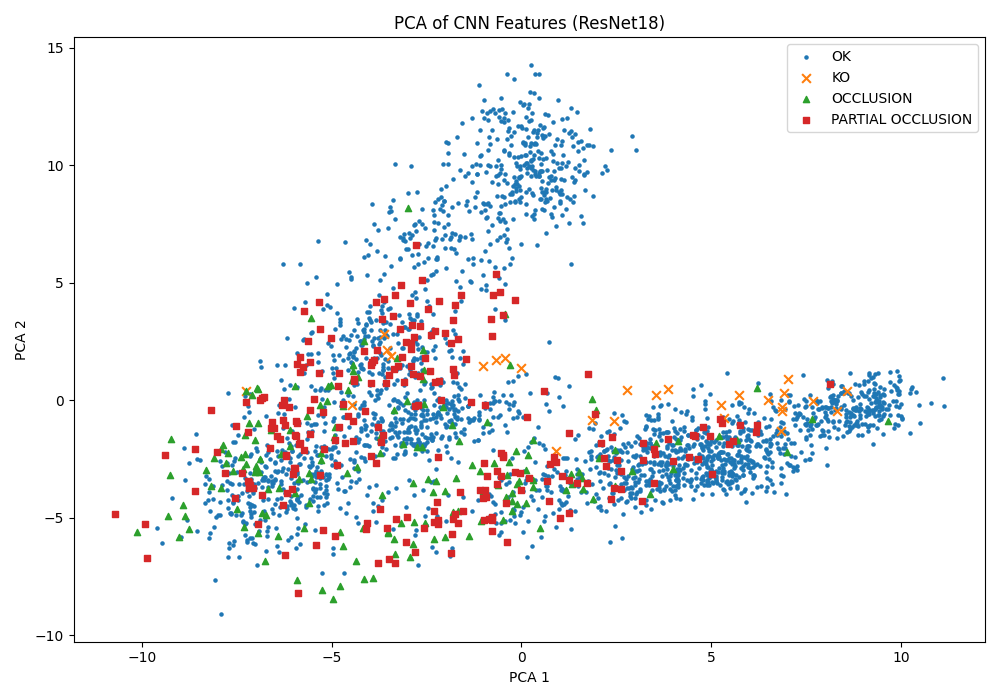
\includegraphics[width=0.7\textwidth]{figures/pca_scatter.png}
    \caption{PCA scatter plot of ResNet18 embeddings. OK samples (blue) form a broad manifold; KO samples (orange) shift slightly outside it; OCCLUSION (green) and PARTIAL OCCLUSION (red) overlap with the OK region.}
    \label{fig:pca}
\end{figure}

The scatter plot revealed several key structural patterns. OK samples form one broad, continuous cluster, confirming that the CNN embeddings capture normal variability across connectors, lighting conditions and board instances. KO samples appear as small groups slightly outside the OK manifold; since they are rare and visually subtle, they shift away from but do not cleanly separate from the OK cluster. OCCLUSION and PARTIAL OCCLUSION samples lie inside the OK region because occlusions alter local appearance without changing the overall connector geometry. The first principal component (PCA1) correlated with brightness, contrast and cable clutter, while PCA2 captured connector cavity depth, vertical shading and perspective variation.

\textbf{PatchCore anomaly detection.} PatchCore~\cite{roth2022patchcore} models only the appearance of normal (OK) data and flags deviations from that learned normality. It extracts intermediate feature maps from ResNet18 (up to \texttt{layer2}), producing spatial feature tensors $\mathbf{F} \in \mathbb{R}^{128 \times H_f \times W_f}$. 

These features are flattened into patch descriptors $\mathcal{P} = \{\mathbf{p}_1, \dots, \mathbf{p}_N\}$ with $\mathbf{p}_i \in \mathbb{R}^{128}$. Each patch represents a small local region capturing geometry, cable edges, shadows and cavity texture. The memory bank stores only OK patches: (1) extract and normalize each patch $\hat{\mathbf{p}} = \mathbf{p} / \|\mathbf{p}\|$; (2) apply coreset sampling to reduce millions of patches to approximately 50,000 representative samples $M = \{\mathbf{m}_1, \dots, \mathbf{m}_K\}$. 

For a test image, each patch is compared to the nearest memory entry and the anomaly score takes the maximum deviation:
\begin{equation}
    d(\mathbf{p}) = \min_{\mathbf{m} \in M} \|\mathbf{p} - \mathbf{m}\|_2, \qquad S = \max_{\mathbf{p} \in \mathcal{P}} d(\mathbf{p})
\end{equation}
A single strongly deviating region is therefore sufficient to classify the entire connector as anomalous. Patch-level distances are rearranged into a spatial anomaly heatmap where bright regions indicate patches that deviate strongly from the OK memory bank.

\textbf{Results.} Evaluation on the full labelled dataset ($N = 453$ scored images) showed that all 27 KO cases were correctly detected as anomalous, with only 8 OK samples becoming false positives. However, 171 full occlusions and 247 partial occlusions were also flagged as anomalous because, from the perspective of patch-level deviation, an occluding cable and a missing cable both look ``different from normal.''

\textbf{Downstream KO-vs-Occlusion classification.} To separate true defects from benign occlusions, a Logistic Regression classifier was trained using only the PatchCore anomaly score $S$ as input. Results were poor (KO F1-score: 0.09, KO recall: 0.25) because the scalar anomaly score alone does not carry enough information to distinguish the type of anomaly. This confirmed that a two-stage design is necessary: an anomaly detector alone cannot solve the three-class problem.

\textbf{Limitations motivating Phase 2.} Five core limitations drove the transition away from PatchCore. First, the memory bank of $\sim$50{,}000 patch embeddings per connector consumes significant RAM and becomes impractical when scaling to all nine connectors (nine banks, nine full $k$-NN search pipelines). Second, inference is slow because each test image requires millions of patch-to-memory distance computations. Third, PatchCore stores features but does not learn a dataset-specific representation, making it sensitive to illumination changes and connector variation. Fourth, the noisy patch-level distance maps produce unstable localization under shadows, reflections or low-contrast conditions. Fifth, and most critically, it cannot distinguish KO from OCCLUSION without an additional classifier that proved unreliable.

\subsection{Phase 2: EfficientAD Teacher-Student Framework}

The second phase (led by Karim Negm) explored EfficientAD~\cite{batzner2023efficientad}, a state-of-the-art teacher-student anomaly detection framework that addresses PatchCore's efficiency limitations while offering sub-5\,ms inference latency.

\textbf{Architecture.} EfficientAD employs two networks. The \emph{Teacher} is a frozen ResNet18 pretrained on ImageNet, serving as a fixed feature extractor. The \emph{Student} is a randomly initialised ResNet18 with identical architecture, trained to mimic the Teacher's feature maps on OK images only. 

At test time, the squared difference between Teacher and Student feature maps is averaged across channels to produce a low-resolution anomaly map. The maximum value of this map becomes the scalar anomaly score. An additional autoencoder branch targets ``logical'' anomalies where a part is visually correct but structurally wrong (e.g.\ a cable routed incorrectly). The published benchmarks report Image-Level AU-ROC of 96.0\% and Pixel-Level AU-PRO of 93.3\% on MVTec AD and LOCO datasets with approximately 4.5\,ms latency per image.

\textbf{Training strategy.} All nine connector types underwent standard training of 70 epochs with intermediate checkpoints saved every 10 epochs for retrospective evaluation. Two input modalities were compared: raw RGB (preserving full colour information) and grayscale with CLAHE enhancement (focusing the network on structural differences). Model selection per connector was automated by a two-criterion logic: (1) primary: minimize false positives on the OK test set; (2) secondary: maximize the margin between the worst OK score and the best KO score. Safety thresholds were computed at 95\% of the minimum defect score.

\textbf{Per-connector results.} The following table summarises the raw RGB modality performance:

\begin{table}[H]
\centering
\small
\begin{tabular}{lccccc}
\toprule
Connector & Recall & Specificity & TP (Caught) & FP (False Alarm) \\
\midrule
conn1 & 1.00 & 1.00 & 5/5 & 0/64 \\
conn2 & 1.00 & 0.97 & 5/5 & 2/64 \\
conn5 & 1.00 & 1.00 & 4/4 & 0/57 \\
conn6 & 0.25 & 0.98 & 1/4 & 1/56 \\
conn7 & 1.00 & 1.00 & 4/4 & 0/59 \\
conn8 & 1.00 & 1.00 & 2/2 & 0/64 \\
conn9 & 1.00 & 0.70 & 2/2 & 20/66 \\
\bottomrule
\end{tabular}
\caption{EfficientAD performance per connector (raw RGB modality).}
\label{tab:efficientad_results}
\end{table}

\begin{figure}[H]
    \centering
    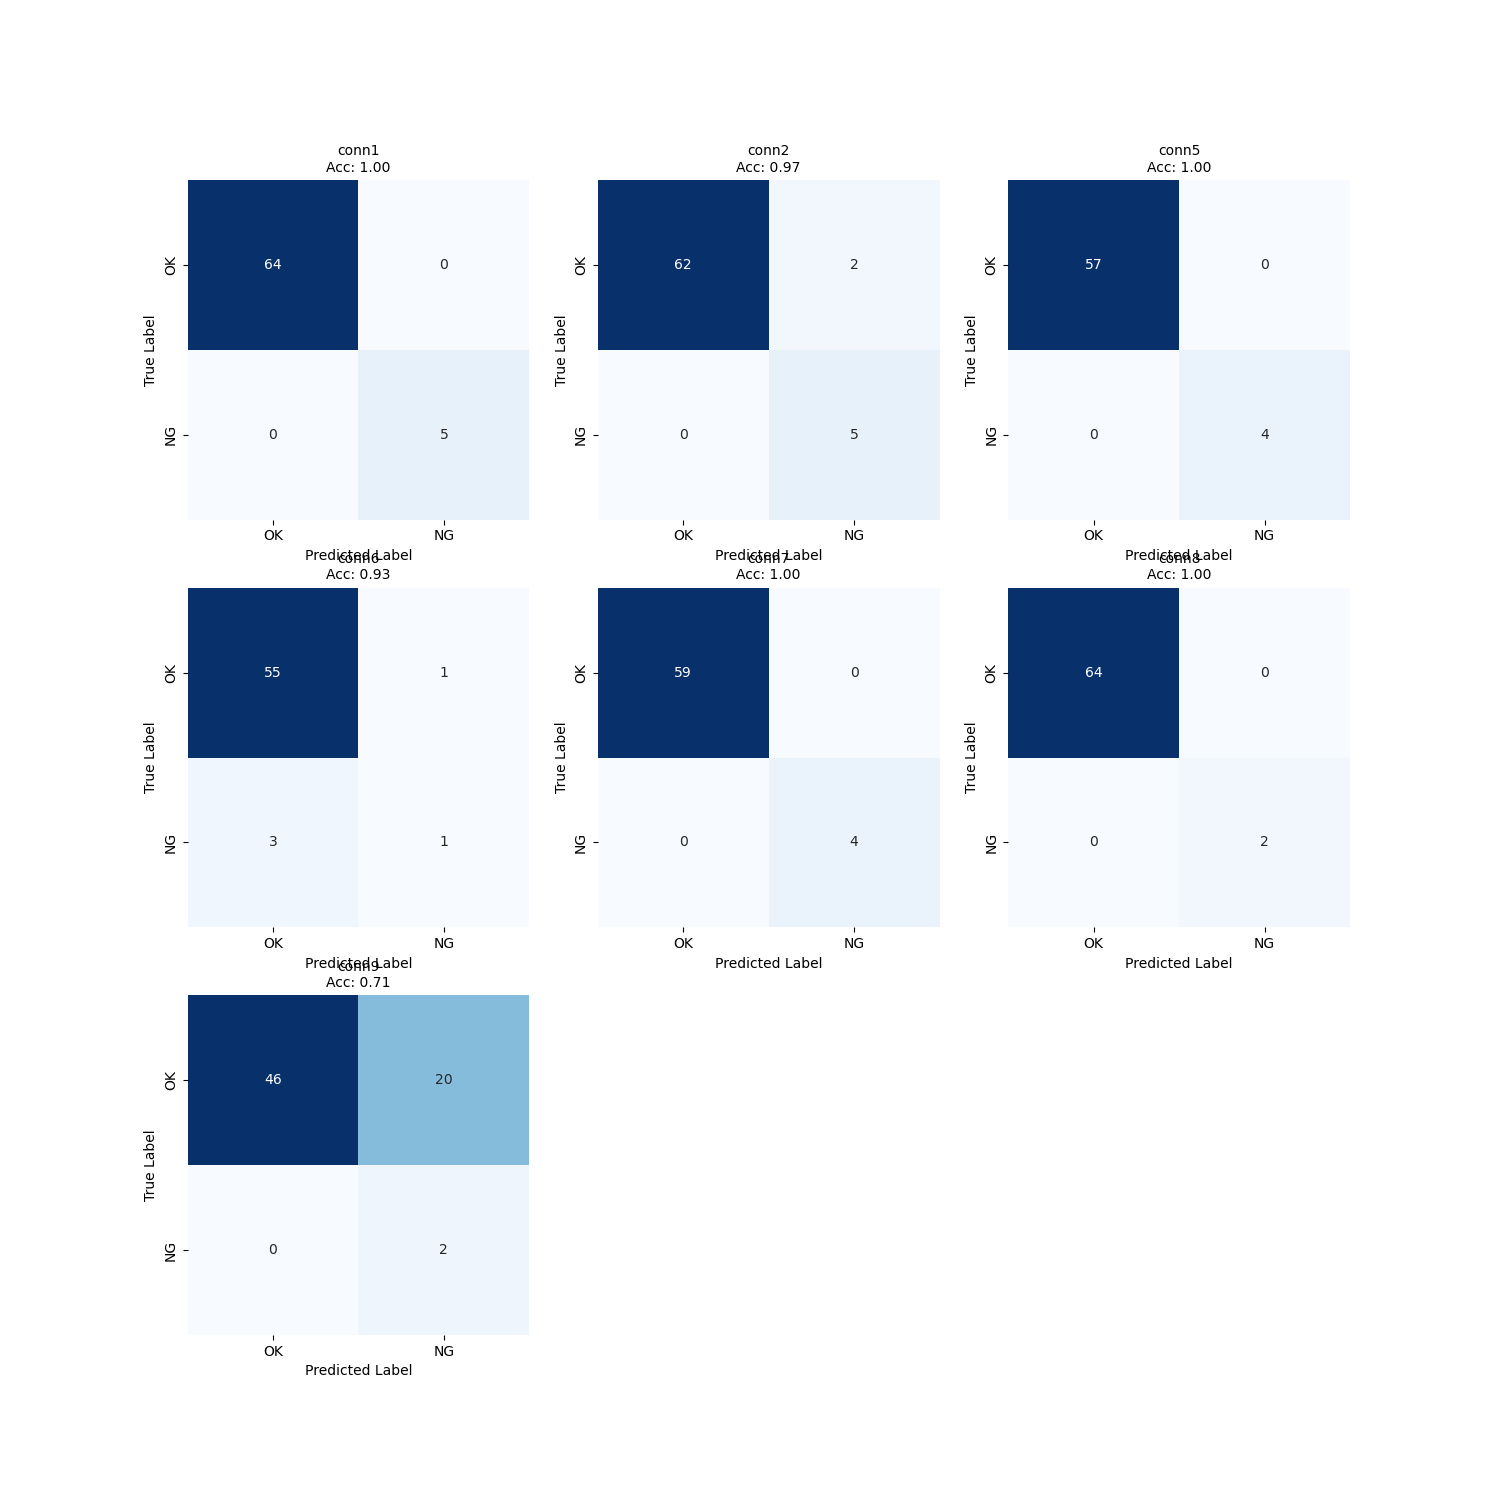
\includegraphics[width=0.85\textwidth]{figures/confusion_matrices.png}
    \caption{EfficientAD confusion matrices. Perfect diagonal separation on conn1, conn5, conn7 and conn8. Conn9 shows 20 false positives; conn6 shows 3 missed defects.}
    \label{fig:efficientad_conf}
\end{figure}

Connectors 1, 5, 7 and 8 achieved perfect recall with zero false positives. However, two failure modes emerged that proved difficult to resolve within the anomaly detection paradigm.

\textbf{Conn6 (low recall, 0.25).} Three out of four defective samples were misclassified as OK. Score distribution analysis revealed that the anomaly scores for these defects were extremely low, overlapping significantly with the normal distribution. This indicated that the Student network had overgeneralised and treated the defect pattern as normal noise. The connector's PCL region is small relative to the background, so the small defect signal gets lost in the larger non-informative area.

\textbf{Conn9 (low specificity, 0.70).} Twenty out of sixty-six OK samples were incorrectly flagged as anomalous. The OK score distribution exhibited a long tail that extended past the safety threshold. Visual inspection suggested that these outliers contained partial occlusions or lighting noise, which the anomaly detector could not distinguish from true structural defects.

\textbf{Multi-step system (Phase 2b).} Building on Phase 2's insights, a multi-step pipeline was developed (led by Giovanni Passuello) that added a dedicated Occlusion Classifier in front of EfficientAD. The OcclusionCNN is a lightweight three-block convolutional network that classifies each connector crop as OCCLUSION or VISIBLE. The architecture uses Conv2d $\to$ BatchNorm $\to$ ReLU $\to$ MaxPool blocks, expanding from 32 to 128 channels, followed by a fully connected head with 512 neurons and dropout of 0.5. 

Only VISIBLE crops proceed to EfficientAD for OK/KO classification. This two-stage design achieved 95.13\% overall accuracy on the full 2{,}853-image dataset, with per-class accuracy of 98.16\% for OK, 84.00\% for KO and 81.03\% for OCCLUSION. The dominant error mode was OCCLUSION samples predicted as KO (56 cases, 11.5\% of occlusions), confirming that even with explicit occlusion filtering, partial occlusions visually resemble structural anomalies.

\subsection{Key Insights Carried Forward}

Across both phases, several insights directly shaped the final PCL Presence pipeline:

\begin{enumerate}[nosep]
    \item \textbf{Anomaly detection alone cannot solve the three-class problem.} Both PatchCore and EfficientAD treat everything ``different from OK'' as anomalous, making it inherently difficult to distinguish missing cables from occluding cables.
    \item \textbf{Per-connector models are essential.} A shared model trained across all connectors is dominated by the easiest cases (conn3, conn8) and fails on the hard ones (conn6, conn7). Each connector requires its own decision boundary.
    \item \textbf{The scarcity of real KO data is the binding constraint.} With fewer than 5 defects per connector, no supervised method can learn a robust KO representation directly. The solution must generate training signal from OK data alone.
    \item \textbf{Occlusions must be handled explicitly.} Relying on the anomaly detector to ignore occlusions produces unacceptable false positive rates. Either a dedicated occlusion classifier or a problem formulation that is inherently robust to occlusions is required.
    \item \textbf{Continuous scores enable operational tuning.} Both PatchCore and EfficientAD output continuous anomaly scores, enabling threshold-based sensitivity adjustment without retraining. This property was deliberately preserved in the final pipeline.
\end{enumerate}

These findings motivated the shift from anomaly detection to synthetic negative classification described in Section~4, where the problem is reformulated as binary presence detection using inpainting-generated training data.

\section{Discussion}

\subsection{Why Synthetic Negatives Work}

Synthetic negatives are effective here because the defect has a simple, localised geometric definition: missing content in a known region. Inpainting inside a connector-specific mask produces negatives that preserve the true background texture, connector housing and lighting conditions of each source image. This eliminates the domain gap that would appear if KO images were generated via generic augmentation (e.g.\ random erasing, CutOut) or sourced from a different production batch.

The approach also scales naturally: adding a new connector type requires only defining a polygon mask in \texttt{mask\_config.json} and collecting OK images. No defect images are needed, which is critical in production environments where defects are extremely rare and expensive to collect.

\subsection{Per-Connector Models vs.\ Global Models}

Even with a shared ResNet18 backbone, per-connector training is essential. The decision boundary differs by connector due to different PCL geometry and entry angle, different background textures and plastic patterns and different levels of illumination variation and glare. A single global model trained across all connectors would be dominated by the easiest cases (conn3, conn8) and fail on the hard ones (conn6, conn7). Per-connector training adds modest overhead (nine models $\times$ 11.2M parameters $\approx$ 400\,MB total on disk) but ensures that each model specialises in the visual signature of its specific connector.

\subsection{Threshold Calibration as Operational Control}

Calibrating $\tau$ from real OK validation images provides a production-oriented control mechanism. If the plant wants fewer false positives, $\tau$ can be increased by choosing a higher percentile (e.g.\ $p=99.9$). If greater sensitivity is required, $\tau$ can be lowered (e.g.\ $p=98$). This change is a deployment parameter requiring no retraining, making it suitable for operational tuning by plant engineers without machine learning expertise.

The continuous $P_{\mathrm{KO}}$ output also supports a \emph{grey zone} workflow: samples with $P_{\mathrm{KO}}$ near $\tau$ (borderline cases) can be flagged for mandatory human review, while samples far from $\tau$ in either direction receive automated pass/fail decisions. This stratified approach maximises throughput while maintaining safety margins.

\subsection{Comparison with Prior Approaches}

\begin{table}[H]
\centering
\small
\begin{tabular}{lcccl}
\toprule
Method & Accuracy & Inference & Memory & Key Limitation \\
\midrule
PatchCore & N/A & Seconds/board & $\sim$50K patches/conn & No KO/OCC separation \\
EfficientAD & Mixed & $<$5\,ms/conn & $\sim$43\,MB/conn & Inconsistent recall \\
\textbf{PCL Presence} & \textbf{95.13\%} & $<$50\,ms/conn & $\sim$45\,MB/conn & Requires mask definition \\
\bottomrule
\end{tabular}
\caption{Comparison of explored approaches.}
\label{tab:comparison}
\end{table}

The PCL Presence pipeline achieves the best trade-off between accuracy, inference speed, memory footprint and operational simplicity. PatchCore's perfect recall came at prohibitive computational cost and without KO/OCCLUSION disambiguation. EfficientAD showed promising results on some connectors but was unreliable on conn6 (25\% recall) and conn9 (30\% FPR). The synthetic negative approach eliminates the need for real KO training data entirely, which is the most practical advantage in a production environment with $<$1\% defect rate.

\subsection{Limitations and Future Improvements}

The current pipeline assumes that the masked region is visually informative. When visibility is degraded due to obstruction, shadows or blur, the classifier produces elevated $P_{\mathrm{KO}}$ even for OK samples, since the visual evidence supporting ``cable present'' is weakened. This reflects genuinely missing information in the image rather than a conceptual failure of the model. The solution is upstream: improved camera placement or additional views to reduce obstruction.

Additionally, the synthetic KO generation assumes that inpainting produces a realistic approximation of an empty connector. For connectors where the cable significantly alters the surrounding texture (e.g.\ through shadow or colour bleed), the synthetic/real domain gap may increase, reducing classifier performance.

Practical upgrades for the next development cycle include: improved camera placement or additional views to reduce obstruction on conn6 and conn7; closed-loop data collection where operator-verified cases are added to the OK training pool; periodic mask refinement driven by false positive heatmaps and borderline $P_{\mathrm{KO}}$ analysis; investigation of lightweight architectures (MobileNetV3, EfficientNet-B0) to reduce per-model memory footprint below 10\,MB.


\section{Conclusions}

The final solution delivers a scalable connector presence detector trained exclusively from real OK samples augmented with realistic synthetic KO images generated by inpainting within connector-specific masks. This converts an extreme-rarity defect detection task into a standard supervised binary classification problem while keeping training data requirements aligned with industrial constraints.

By combining per-connector ResNet18 models with conservative percentile-based threshold calibration on real OK validation data, the system provides reliable decisions and interpretable probabilities that support production deployment. The approach is lightweight ($\sim$400\,MB total), reproducible (fixed seeds, saved artefacts) and maintainable (adding a connector requires only a mask definition and OK images), making it suitable for long-term use in a factory environment where data drift and hardware changes are expected.

\section{Acknowledgments}

We sincerely thank \textbf{Prof.\ Fredy Ruiz} for his guidance on balancing technical rigour with deployability. We are deeply grateful to \textbf{Marco Cederle} and \textbf{Davide Cazzaniga} from Beko Europe for their domain expertise and for facilitating our factory visits. Special thanks to the production operators for their practical feedback on our interface.

\begin{thebibliography}{9}

\bibitem{batzner2023efficientad}
K.~Batzner, L.~Heckler and R.~K\"onig, ``EfficientAD: Accurate Visual Anomaly Detection at Millisecond-Level Latencies,'' \textit{arXiv preprint arXiv:2303.14535}, 2023.

\bibitem{rublee2011orb}
E.~Rublee, V.~Rabaud, K.~Konolige and G.~Bradski, ``ORB: An efficient alternative to SIFT or SURF,'' \textit{Proc.\ ICCV}, 2011.

\bibitem{roth2022patchcore}
K.~Roth, L.~Pemula, J.~Zepeda, B.~Sch\"olkopf, T.~Brox and P.~Gehler, ``Towards Total Recall in Industrial Anomaly Detection,'' \textit{Proc.\ IEEE/CVF CVPR}, 2022.

\bibitem{he2016resnet}
K.~He, X.~Zhang, S.~Ren and J.~Sun, ``Deep Residual Learning for Image Recognition,'' \textit{Proc.\ IEEE CVPR}, 2016.

\bibitem{pizer1987clahe}
S.~M.~Pizer \textit{et al.}, ``Adaptive histogram equalization and its variations,'' \textit{Computer Vision, Graphics, and Image Processing}, vol.~39, no.~3, pp.~355--368, 1987.

\bibitem{telea2004inpainting}
A.~Telea, ``An Image Inpainting Technique Based on the Fast Marching Method,'' \textit{Journal of Graphics Tools}, vol.~9, no.~1, pp.~23--34, 2004.

\bibitem{selvaraju2017gradcam}
R.~R.~Selvaraju, M.~Cogswell, A.~Das, R.~Vedantam, D.~Parikh and D.~Batra, ``Grad-CAM: Visual Explanations from Deep Networks via Gradient-based Localization,'' \textit{Proc.\ IEEE ICCV}, 2017.

\end{thebibliography}

\end{document}